\documentclass[10pt, aspectratio=169]{beamer}
\definecolor{CustomNavy}{RGB}{0, 51, 102}
\definecolor{CustomBlue}{RGB}{41, 128, 185}
\definecolor{CustomGray}{RGB}{100, 110, 120}
\definecolor{CustomDark}{RGB}{40, 40, 40}
\usetheme{default}
\usecolortheme{default}
\setbeamertemplate{navigation symbols}{}
\usepackage[utf8]{inputenc}
\usepackage[T1]{fontenc}
\usepackage{helvet}
\renewcommand{\familydefault}{\sfdefault}
\setbeamercolor{title}{fg=CustomNavy}
\setbeamercolor{frametitle}{fg=CustomNavy}
\setbeamercolor{subtitle}{fg=CustomGray}
\setbeamercolor{author}{fg=CustomDark}
\setbeamercolor{institute}{fg=CustomGray}
\setbeamercolor{block title}{bg=CustomNavy, fg=white}
\setbeamercolor{block body}{bg=CustomNavy!5, fg=CustomDark}
\setbeamertemplate{title page}{
	\vbox{}
	\vfill
	\begin{raggedright}
		{\usebeamerfont{title}\usebeamercolor[fg]{title}\Large\bfseries\inserttitle}\par\vspace{0.25cm}
		\ifx\insertsubtitle\@empty\else
		{\usebeamerfont{subtitle}\usebeamercolor[fg]{subtitle}\small\insertsubtitle}\par\vspace{0.4cm}
		\fi
		{\color{CustomBlue}\hrule height 0.75pt width 0.35\linewidth}\par\vspace{0.4cm}
		{\usebeamerfont{author}\usebeamercolor[fg]{author}\textbf{\insertauthor}}\par\vspace{0.1cm}
		{\usebeamerfont{institute}\usebeamercolor[fg]{institute}\footnotesize\insertinstitute}\par
	\end{raggedright}
	\vfill
}
\title{What Is Globalization?}
\subtitle{And How Has the Global Economy Shaped the United States?}
\author{Nagaraj}
\institute{Department of Economics}
\date{}
\begin{document}
	
	\begin{frame}
		\titlepage
	\end{frame}
	
	\begin{frame}{Globalization and the U.S. Economy}{Background \& Key Questions}
		\begin{itemize}
			\item Technological, logistics, and policy advances over centuries have created an \textbf{unprecedentedly integrated} global marketplace.
			\vspace{0.25cm}
			\item The central macro debate centers on whether economic integration yields \textbf{net welfare gains} or creates structural domestic losses.
			\vspace{0.25cm}
			\item Differential shocks impact three key economic sectors:
			\begin{itemize}
				\vspace{0.1cm}
				\item \textbf{Firms:} Rapid market expansion versus heightened foreign price competition.
				\item \textbf{Labor:} Gains from high-skill specialization versus displacement in trade-exposed sectors.
				\item \textbf{Households:} Purchasing power gains and product variety versus global supply shocks.
			\end{itemize}
		\end{itemize}
		
		\vspace{0.3cm}
		
		\begin{block}{Analytical Goal}
			Evaluate the empirical trade-offs and distribution of economic gains across the domestic economy.
		\end{block}
	\end{frame}
	
	\begin{frame}{Defining Globalization}{Scope, History, and Core Trade-Offs}
		\begin{itemize}
			\item Characterized by the growing \textbf{cross-border interdependence} of national markets through trade, financial investment, technology transfers, and labor mobility.
			\vspace{0.25cm}
			\item Accelerated significantly during the post-Cold War expansion of open market institutions in the 1990s.
			\vspace{0.25cm}
			\item Generates substantial aggregate gains in efficiency, scale, and capital allocation, but introduces significant \textbf{distributional trade-offs}:
			\begin{itemize}
				\vspace{0.1cm}
				\item Facilitates innovation diffusion, cost reduction, and market expansion.
				\item Induces local labor market frictions, supply chain vulnerabilities, and geopolitical exposure.
			\end{itemize}
			\vspace{0.25cm}
			\item Maximizing social welfare requires policies that capture global efficiency gains while mitigating regional and sectoral disruptions.
		\end{itemize}
	\end{frame}
	
	\begin{frame}{Historical Waves of Global Integration}{Technology, Infrastructure, and Policy Regimes}
		\begin{itemize}
			\item Early trade was constrained by transport frictions, but the \textbf{first major wave} took off in the $19^{\text{th}}$ century driven by steamships, railways, telegraphs, and imperial trade networks.
			\vspace{0.25cm}
			\item This first era of integration collapsed dramatically due to the major macroeconomic and political shocks of \textbf{World War I, interwar protectionism, the Great Depression, and World War II}.
			\vspace{0.25cm}
			\item A \textbf{second wave} emerged post-1945 under U.S. institutional leadership, establishing rules-based multilateral frameworks to rebuild international trade and capital flows.
			\vspace{0.25cm}
			\item While ongoing, contemporary global integration faces heightened headwinds from cyclical downturns, financial instability, and rising geopolitical scrutiny.
		\end{itemize}
	\end{frame}
	
	\begin{frame}{Technological Breakthroughs and Industrialization}{1800--1899}
		\begin{itemize}
			\item Steamships, railways, and telegraphs lowered transport and transaction costs, accelerating industrial mass production and global market integration.
			\vspace{0.25cm}
			\item Adoption of the Gold Standard stabilized foreign exchange rates, minimizing currency risks and stimulating international capital movement.
			\vspace{0.25cm}
			\item Western powers established colonial resource extraction networks and forced open trade access across East Asian economies.
		\end{itemize}
	\end{frame}
	
	\begin{frame}{Transport Innovations and the First World War}{1900--1918}
		\begin{itemize}
			\item Commercial adoption of automobiles and transoceanic aviation further enhanced international connectivity and reduced regional transit friction.
			\vspace{0.25cm}
			\item Outbreak of World War I severely disrupted international trade flows and destabilized global commercial and financial networks.
			\vspace{0.25cm}
			\item Severe post-war reparation obligations imposed on Germany destabilized European economic recovery and heightened fiscal strain.
		\end{itemize}
	\end{frame}
	
	\begin{frame}{Interwar Instability and the Great Depression}{1920--1939}
		\begin{itemize}
			\item Interwar Gold Standard reinstatement, asset bubble expansion, and German hyperinflation fueled acute macroeconomic volatility.
			\vspace{0.25cm}
			\item The 1929 stock market crash triggered global depression, leading nations to abandon currency pegs and pursue competitive devaluations.
			\vspace{0.25cm}
			\item Trade retaliation following the U.S. Smoot-Hawley Tariff fragmented the global economy into isolated, protectionist regional blocs.
		\end{itemize}
	\end{frame}
	
	\begin{frame}{World War II and the Bretton Woods Architecture}{1939--1945}
		\begin{itemize}
			\item World War II mobilized industrial capacities globally while temporarily severing normal international commercial channels.
			\vspace{0.25cm}
			\item The 1944 Bretton Woods conference established a rules-based monetary order centered on a gold-pegged U.S. dollar to promote postwar recovery and trade liberalization.
			\vspace{0.25cm}
			\item Non-ratification by the Soviet Union and subsequent Cold War tensions divided global commerce into Western market integration and an isolated Eastern bloc.
		\end{itemize}
	\end{frame}
	
	\begin{frame}{Multilateral Trade Liberalization and Computing}{1948--1969}
		\begin{itemize}
			\item Inception of the General Agreement on Tariffs and Trade (GATT) in 1948 established the first worldwide multilateral framework for open commercial exchange.
			\vspace{0.25cm}
			\item Early computing innovations laid the groundwork for advanced data processing and modern commercial breakthroughs.
			\vspace{0.25cm}
			\item The Kennedy Round of GATT negotiations further accelerated tariff reductions and expanded global trade liberalization.
		\end{itemize}
	\end{frame}
	
	\begin{frame}{End of Fixed Exchange Rates and Oil Shocks}{1970--1979}
		\begin{itemize}
			\item Energy price spikes by the Organization of the Petroleum Exporting Countries (\textbf{OPEC}) triggered high inflation and unemployment across the global economy.
			\vspace{0.25cm}
			\item U.S. inflation and growing trade imbalances compelled the Nixon administration to end dollar convertibility to gold for foreign governments, leading most currencies to adopt \textbf{floating exchange rates}.
			\vspace{0.25cm}
			\item These macroeconomic shocks disrupted postwar stability and forced nations to adapt to new monetary and energy realities.
		\end{itemize}
	\end{frame}
	
	\begin{frame}{Debt Crisis, Free Markets, and the Plaza Accord}{1980--1989}
		\begin{itemize}
			\item The IMF and international institutions imposed strict austerity and free-market policies on Latin American nations in exchange for aid, sparking severe local backlash.
			\vspace{0.25cm}
			\item President Ronald Reagan and UK Prime Minister Margaret Thatcher championed deregulation, leading to the rapid rise of Wall Street and \textbf{financial globalization}.
			\vspace{0.25cm}
			\item Mounting U.S. trade deficits—particularly with Japan—culminated in the \textbf{Plaza Accord}, a coordinated foreign exchange intervention to depreciate the U.S. dollar.
		\end{itemize}
	\end{frame}
	
	\begin{frame}{End of the Cold War and Institutional Integration}{1989--1991}
		\begin{itemize}
			\item The collapse of the Soviet Union eliminated geopolitical bipolarity, fostering greater international cooperation across global institutions.
			\vspace{0.25cm}
			\item Former Eastern bloc nations integrated into market economies, rapidly expanding global trade networks and capital flows.
			\vspace{0.25cm}
			\item This era marked the beginning of a truly globalized marketplace driven by unified trade policies and diplomatic alignment.
		\end{itemize}
	\end{frame}
	
	\begin{frame}{The Internet and the Rise of Multinational Corporations}{1990--1999}
		\begin{itemize}
			\item The internet began its meteoric rise, radically transforming global commerce, communication, and information sharing.
			\vspace{0.25cm}
			\item Powerful multinational corporations (MNCs) emerged to dominate the global economy, leveraging cross-border supply chains and digital connectivity.
			\vspace{0.25cm}
			\item Accelerated foreign direct investment (FDI) and digital infrastructure cemented a deeply interconnected worldwide market.
		\end{itemize}
	\end{frame}
	
	\begin{frame}{The European Union and Continental Integration}{1993}
		\begin{itemize}
			\item The formal formation of the \textbf{European Union} in 1993 solidified the single market that began developing in the 1950s.
			\vspace{0.25cm}
			\item The integration process culminated in the establishment of the single \textbf{euro currency} in 1999, deepening economic and monetary union across member states.
			\vspace{0.25cm}
			\item Created one of the world's largest economic blocs, streamlining regulatory standards and eliminating intra-regional trade barriers.
		\end{itemize}
	\end{frame}
	
	\begin{frame}{North American Free Trade Agreement (NAFTA)}{1994}
		\begin{itemize}
			\item A major trilateral trade agreement between \textbf{Canada, Mexico, and the United States} went into force following intense debate within the U.S.
			\vspace{0.25cm}
			\item It marked a historic milestone as the \textbf{first free trade agreement} established between the United States and a developing nation.
			\vspace{0.25cm}
			\item Drastically reduced tariffs and integrated supply chains across North America, while sparking enduring domestic debates regarding labor and manufacturing shifts.
		\end{itemize}
	\end{frame}
	
	\begin{frame}{World Trade Organization (WTO)}{1995}
		\begin{itemize}
			\item The modern, rules-governed global trading system was formally established with the creation of the \textbf{World Trade Organization (WTO)}.
			\vspace{0.25cm}
			\item The WTO replaced the provisional General Agreement on Tariffs and Trade (GATT), providing a permanent institutional framework.
			\vspace{0.25cm}
			\item Introduced a robust dispute settlement mechanism to enforce international trade rules and reduce global trade barriers.
		\end{itemize}
	\end{frame}
	
	\begin{frame}{East Asian Financial Crisis}{1997}
		\begin{itemize}
			\item Sharp declines in Asian currencies triggered a severe financial crisis across the region, exposing vulnerabilities in fixed exchange rate regimes.
			\vspace{0.25cm}
			\item Affected countries were forced to accept stringent \textbf{austerity measures} in exchange for emergency international financial bailouts.
			\vspace{0.25cm}
			\item The harsh conditions imposed during the crisis revived widespread local hostility and political backlash toward the \textbf{IMF}.
		\end{itemize}
	\end{frame}
	
	\begin{frame}{China's WTO Accession and the Global Financial Crisis}{2001 \& 2008}
		\begin{itemize}
			\item \textbf{2001 (China and the WTO):} China joined the WTO, becoming the world's largest developing economy after the U.S. granted Permanent Normal Trade Relations in anticipation of greater market openness.
			\vspace{0.25cm}
			\item \textbf{2008 (Global Financial Crisis):} An international banking crash and European debt crisis triggered the worst global recession since the Great Depression.
			\vspace{0.25cm}
			\item The G-20 stepped in as a primary steering committee, but the crisis fueled a broader domestic and political backlash against globalization and U.S. leadership.
		\end{itemize}
	\end{frame}
	
	\begin{frame}{Brexit}{2016 — 2021}
		\begin{itemize}
			\item The United Kingdom votes to leave the European Union, complicating cross-border movement and trade.
			\vspace{0.25cm}
			\item A last-minute deal between the two sides signed in December 2020 allows a continuation of tariff-free trade in goods, but UK-EU trade still falls sharply, and the UK economy suffers after Britain exits the European Union in January 2021, leaving many issues unresolved.
		\end{itemize}
	\end{frame}
	
	\begin{frame}{Trump Presidency Upends US Trade with Allies}{2017 — 2020}
		\begin{itemize}
			\item President Donald J. Trump disrupts the world trading and supply chain system by withdrawing from the Trans-Pacific Partnership (TPP), forcing a more restrictive rewrite of NAFTA, blocking the WTO’s ability to settle trade disputes, and threatening or imposing tariffs on allies like Canada, South Korea, and the European Union citing national security concerns.
		\end{itemize}
	\end{frame}
	
	\begin{frame}{US-China Trade War}{2018}
		\begin{itemize}
			\item Trump ignites a tit-for-tat trade war with China, leading to tariffs covering over half of the goods traded between the two countries by September 2019.
			\vspace{0.25cm}
			\item China’s pledge to expand purchases of certain US goods and services falls short.
			\vspace{0.25cm}
			\item The tariffs remain and in some cases (in advanced technology and electric vehicles) are expanded under President Joseph R. Biden Jr., as of mid-2024.
		\end{itemize}
	\end{frame}
	
	\begin{frame}{COVID-19 Pandemic}{2020 — 2023}
		\begin{itemize}
			\item The SARS-CoV-2 virus spreads worldwide, costing over 6.8 million lives, disrupting global supply chains, and triggering a global recession.
			\vspace{0.25cm}
			\item By the end of 2020, several vaccines are developed and distributed globally, but with uneven access.
			\vspace{0.25cm}
			\item More transmissible variants spur additional outbreaks. The global public health emergency ends in May 2023.
		\end{itemize}
	\end{frame}
	
	\begin{frame}{Russia’s War on Ukraine}{2022 }
		\begin{itemize}
			\item Russian president Vladimir Putin invades Ukraine, triggering a humanitarian crisis and roiling global food and energy markets, prompting more than a thousand multinational companies to scale back or sever business ties with Russia.
			\vspace{0.25cm}
			\item Many countries impose coordinated sanctions on Russia to deter Putin’s war effort.
			\vspace{0.25cm}
			\item Rising energy prices and fears of natural gas exports from Russia to Europe deepen Europe’s economic problems.
		\end{itemize}
	\end{frame}
\begin{frame}{Postwar Trade Integration and Contemporary Deceleration}
\framesubtitle{World trade in goods and services as percent of world GDP, 1870--2023}
    \vspace{-0.2cm}
    \begin{center}
        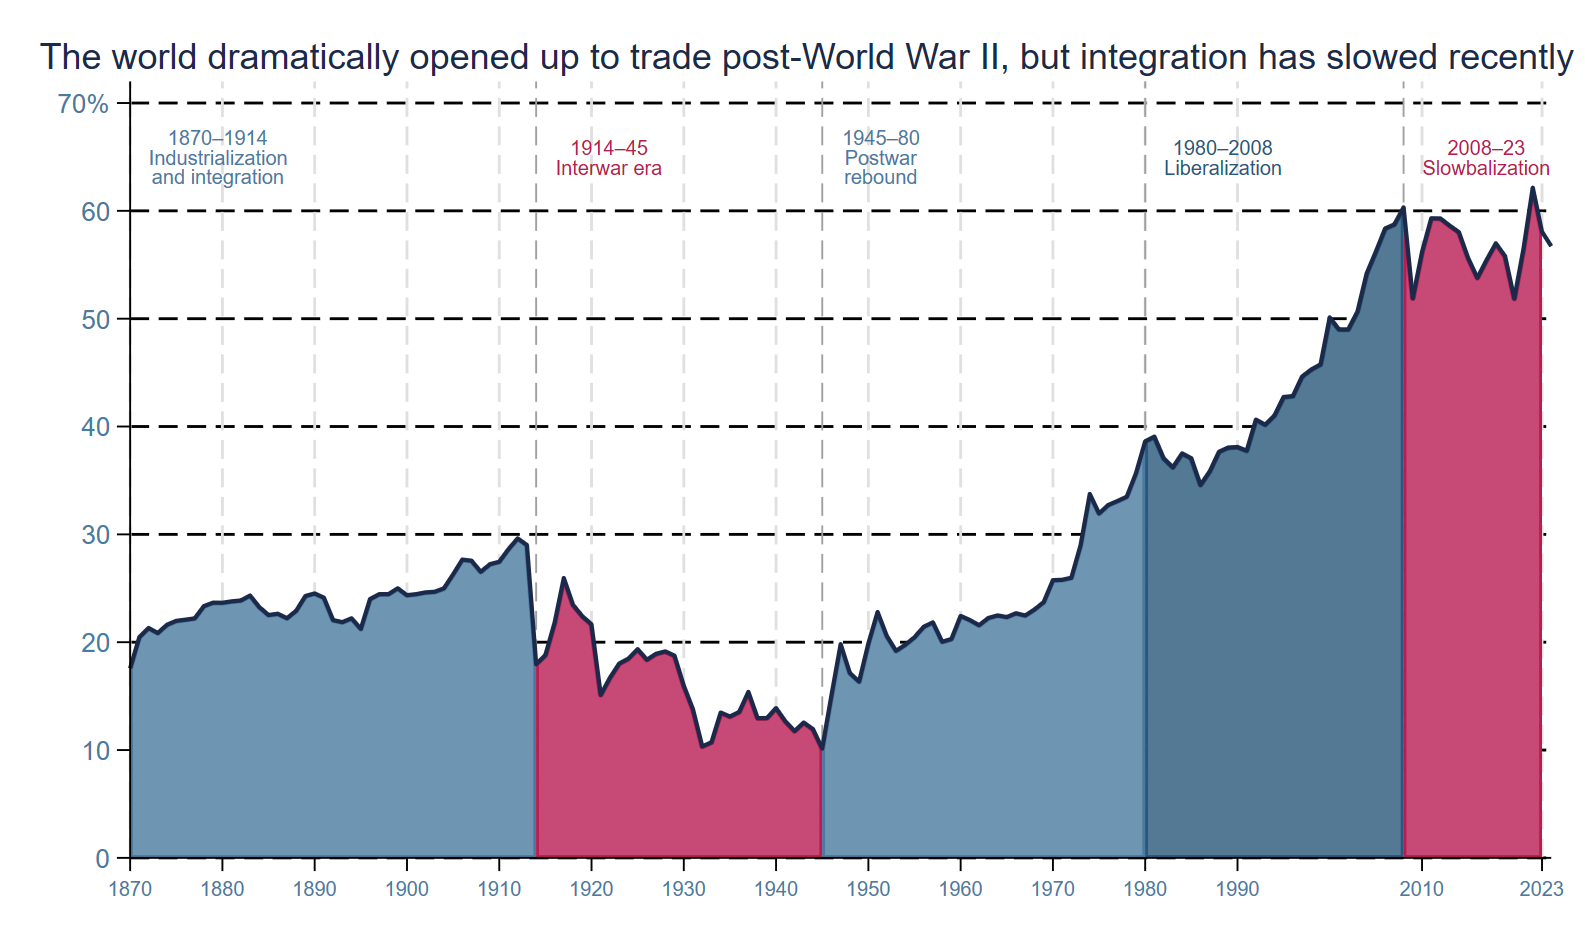
\includegraphics[width=0.96\linewidth, height=0.72\textheight, keepaspectratio]{p1.png}
    \end{center}
    \vfill
    {\tiny \color{CustomGray}\textbf{Source:} Our World in Data (OWID).}
\end{frame}
\begin{frame}
    \vspace{-0.2cm}
    \begin{center}
        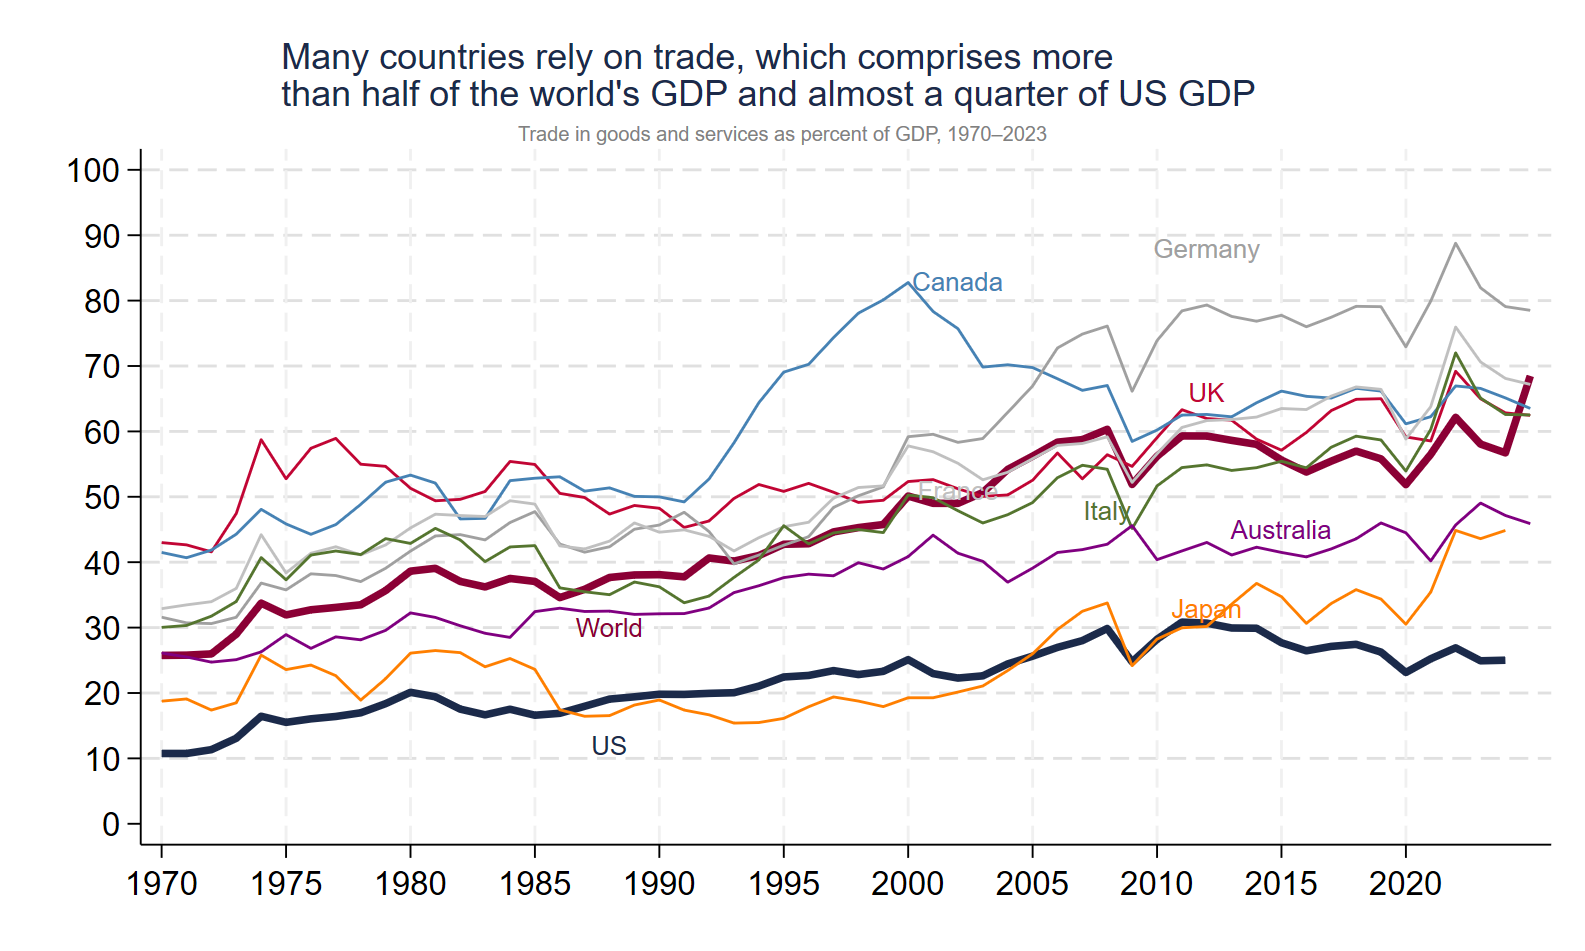
\includegraphics[width=0.98\linewidth, height=0.82\textheight, keepaspectratio]{pic_2.png}
    \end{center}
    \vfill
    {\tiny \color{CustomGray}\textbf{Source:} World Development Indicators (WDI).}
\end{frame}
\begin{frame}
    \vspace{-0.2cm}
    \begin{center}
        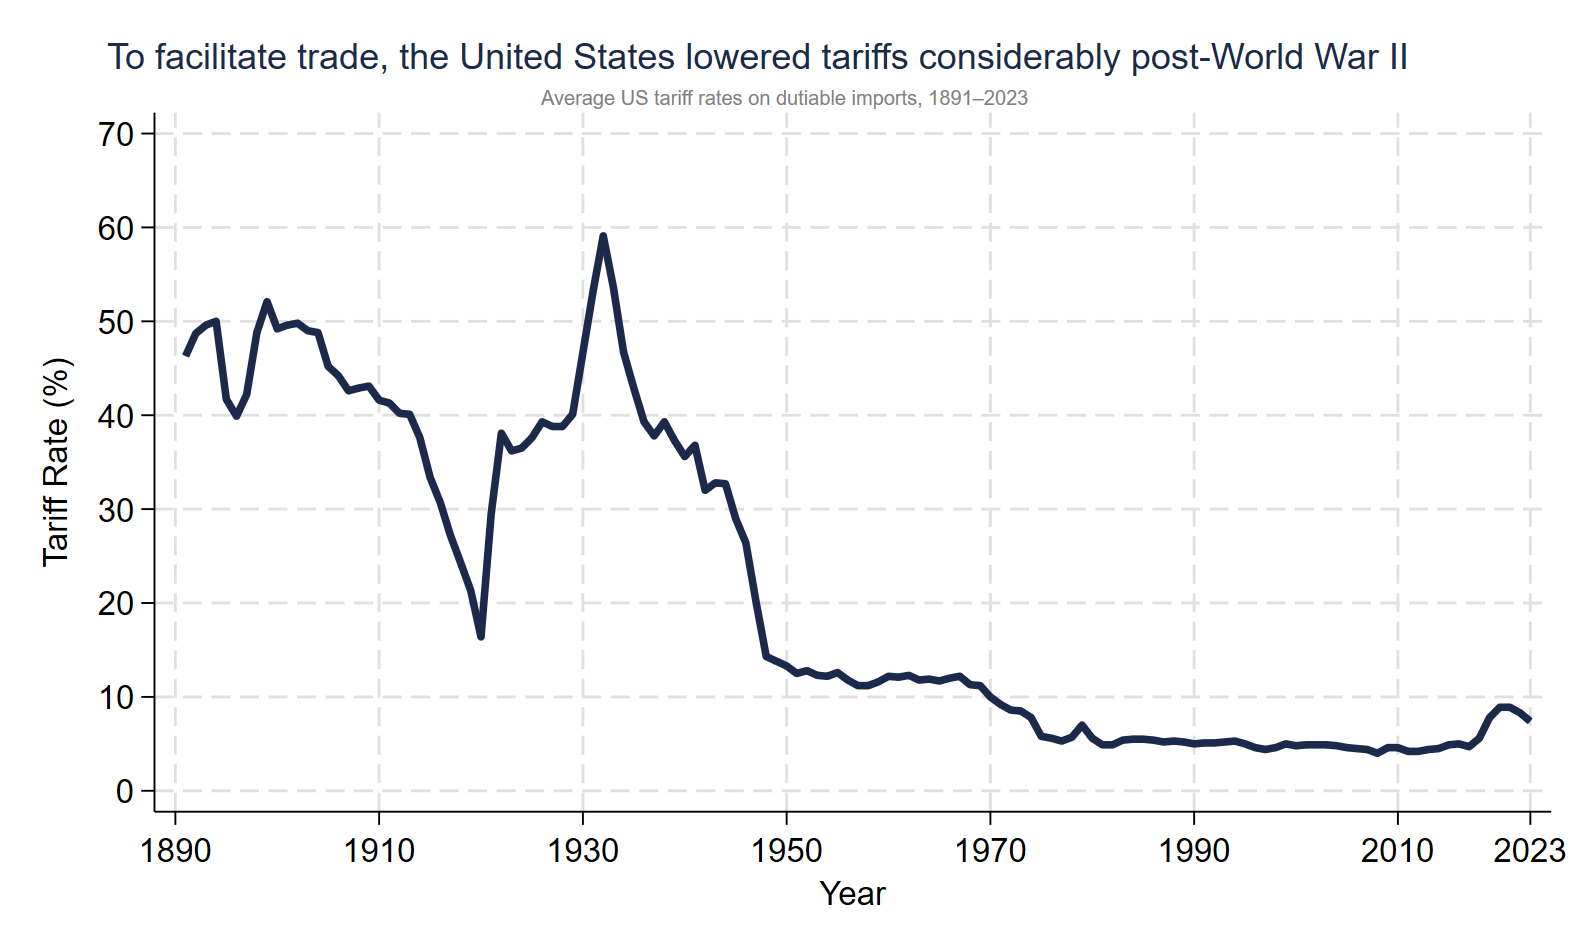
\includegraphics[width=0.98\linewidth, height=0.82\textheight, keepaspectratio]{pic_3.png}
    \end{center}
    \vfill
    {\tiny \color{CustomGray}\textbf{Source:} UN International Trade Commission.}
\end{frame}
\begin{frame}{Tariff Liberalization and Integration in Emerging Economies}
\framesubtitle{Average applied tariff rates, 1988–2022}
    \vspace{-0.3cm}
    \begin{columns}[c]
        % Left Column: Emerging Markets
        \begin{column}{0.48\textwidth}
            \centering
            {\small \textbf{Emerging Markets}}\par\vspace{0.1cm}
            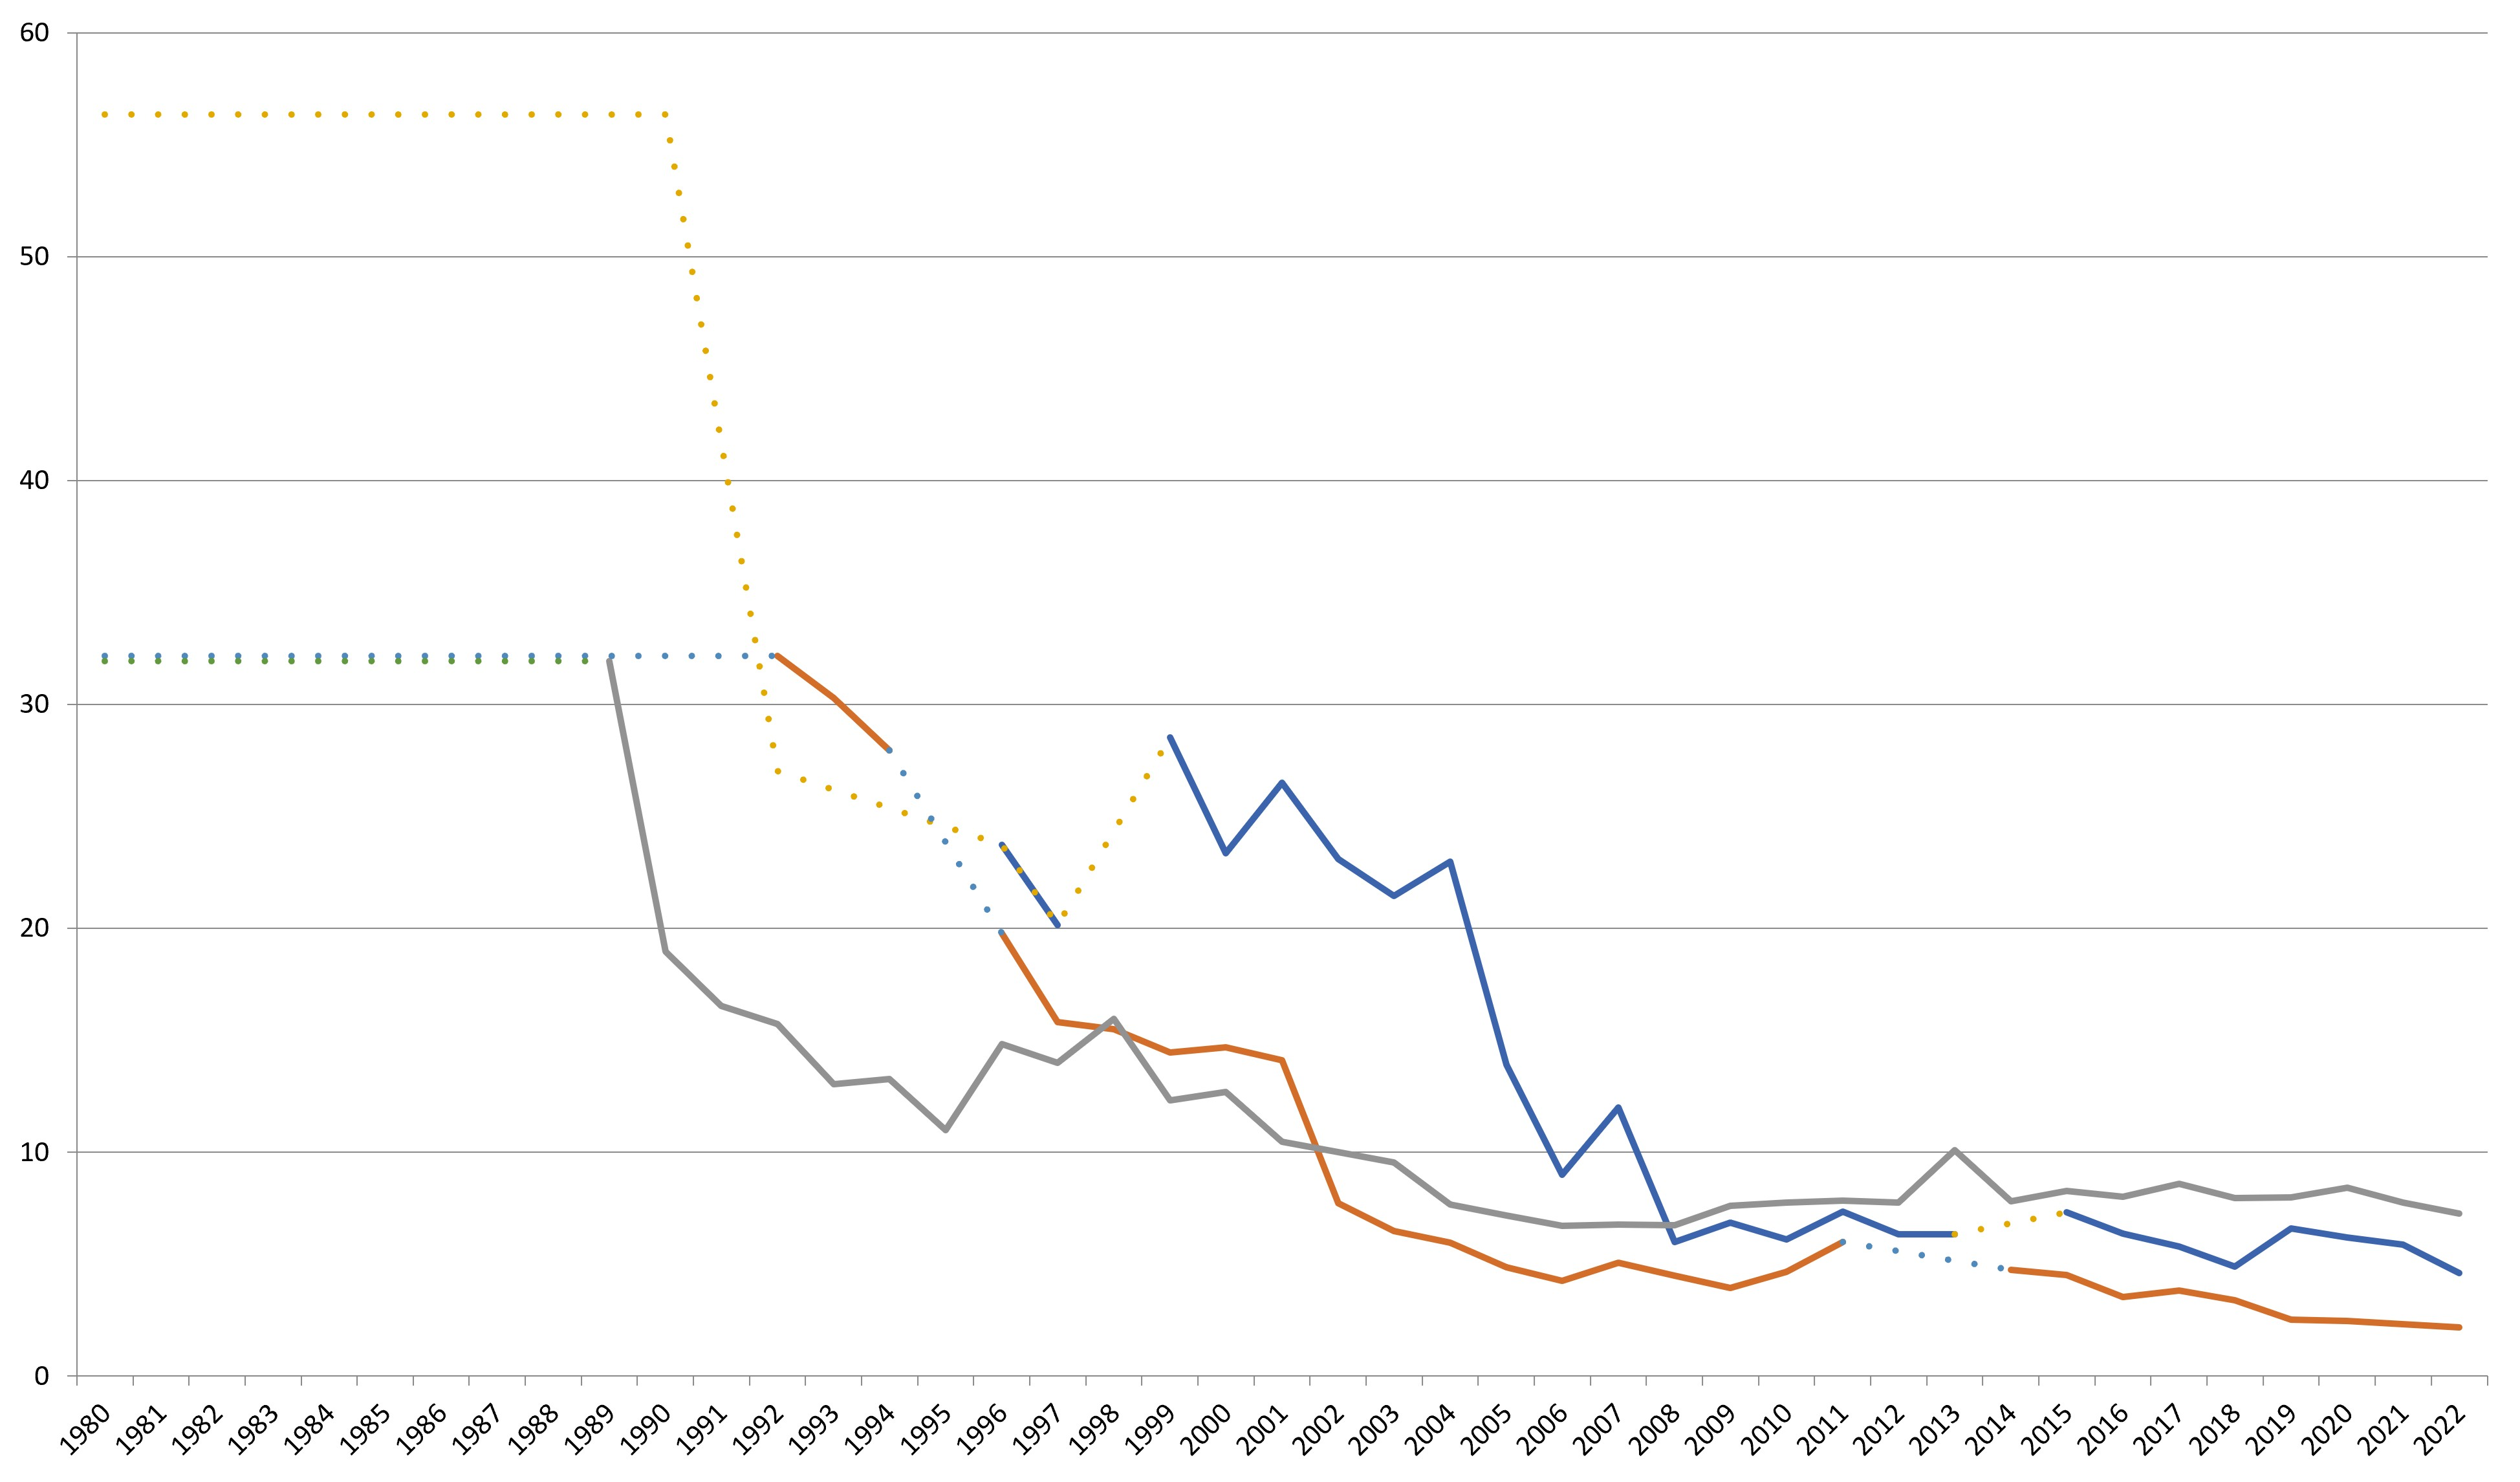
\includegraphics[width=\linewidth, height=0.46\textheight]{pic4.png}
        \end{column}
        % Right Column: Advanced Economies
        \begin{column}{0.48\textwidth}
            \centering
            {\small \textbf{Advanced Economies}}\par\vspace{0.1cm}
            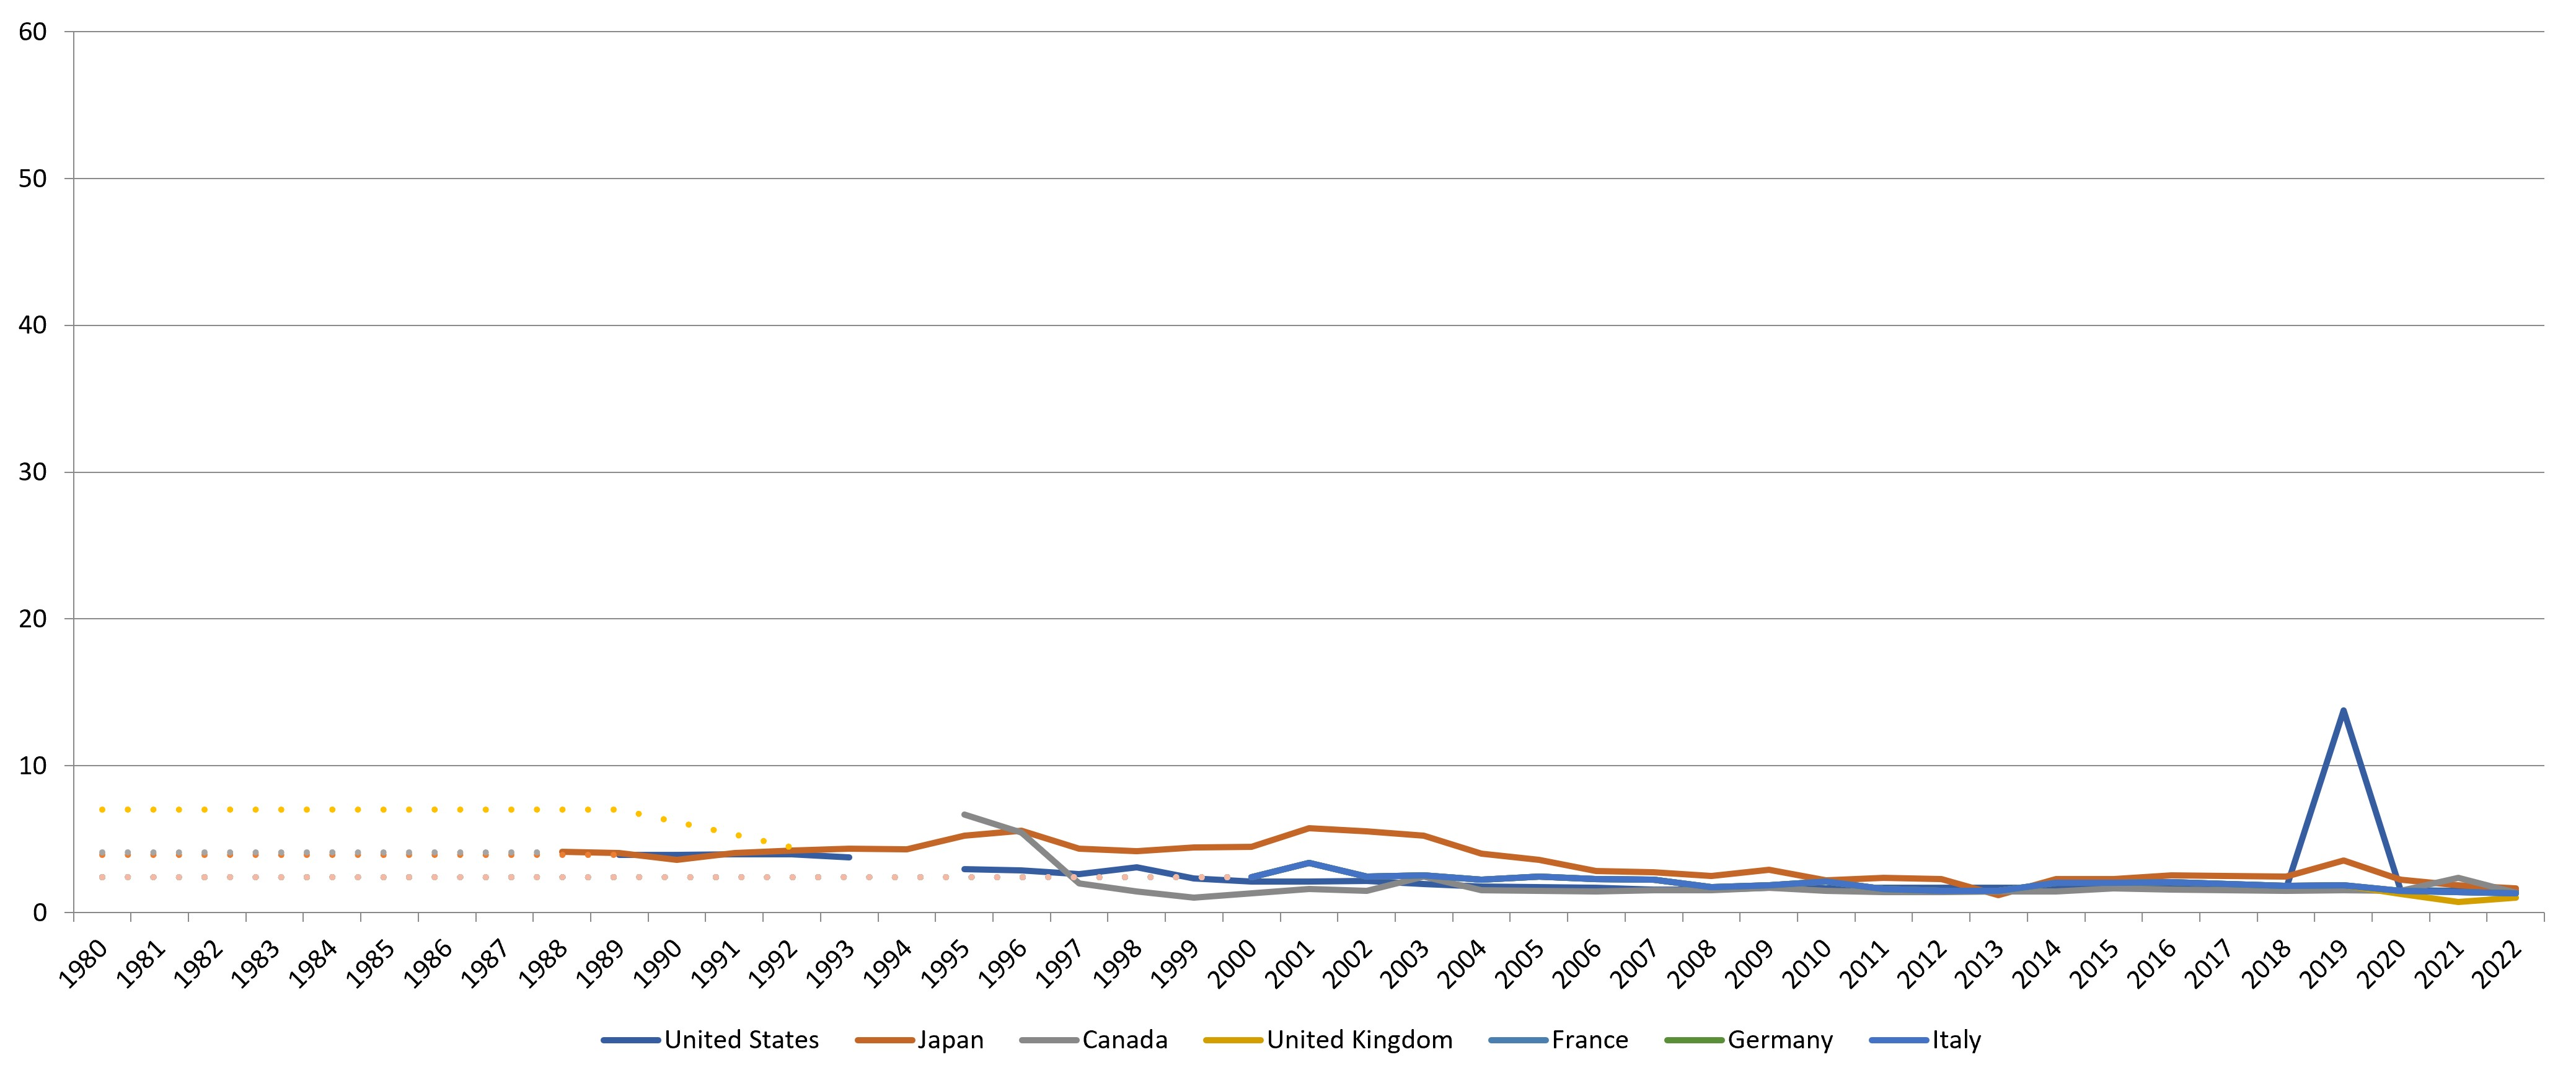
\includegraphics[width=\linewidth, height=0.46\textheight]{pic_4b.png}
        \end{column}
    \end{columns}
    \vfill
    {\tiny \color{CustomGray}\textbf{Note:} Rates are weighted by trade value. Dotted lines indicate when data are not available. Recent data for the United States and China are excluded due to the effects of the US-China trade war on data quality.\par}
    \vspace{0.05cm}
    {\tiny \color{CustomGray}\textbf{Source:} World Development Indicators (WDI).}
\end{frame}
\begin{frame}
    \vspace{-0.2cm}
    \begin{center}
        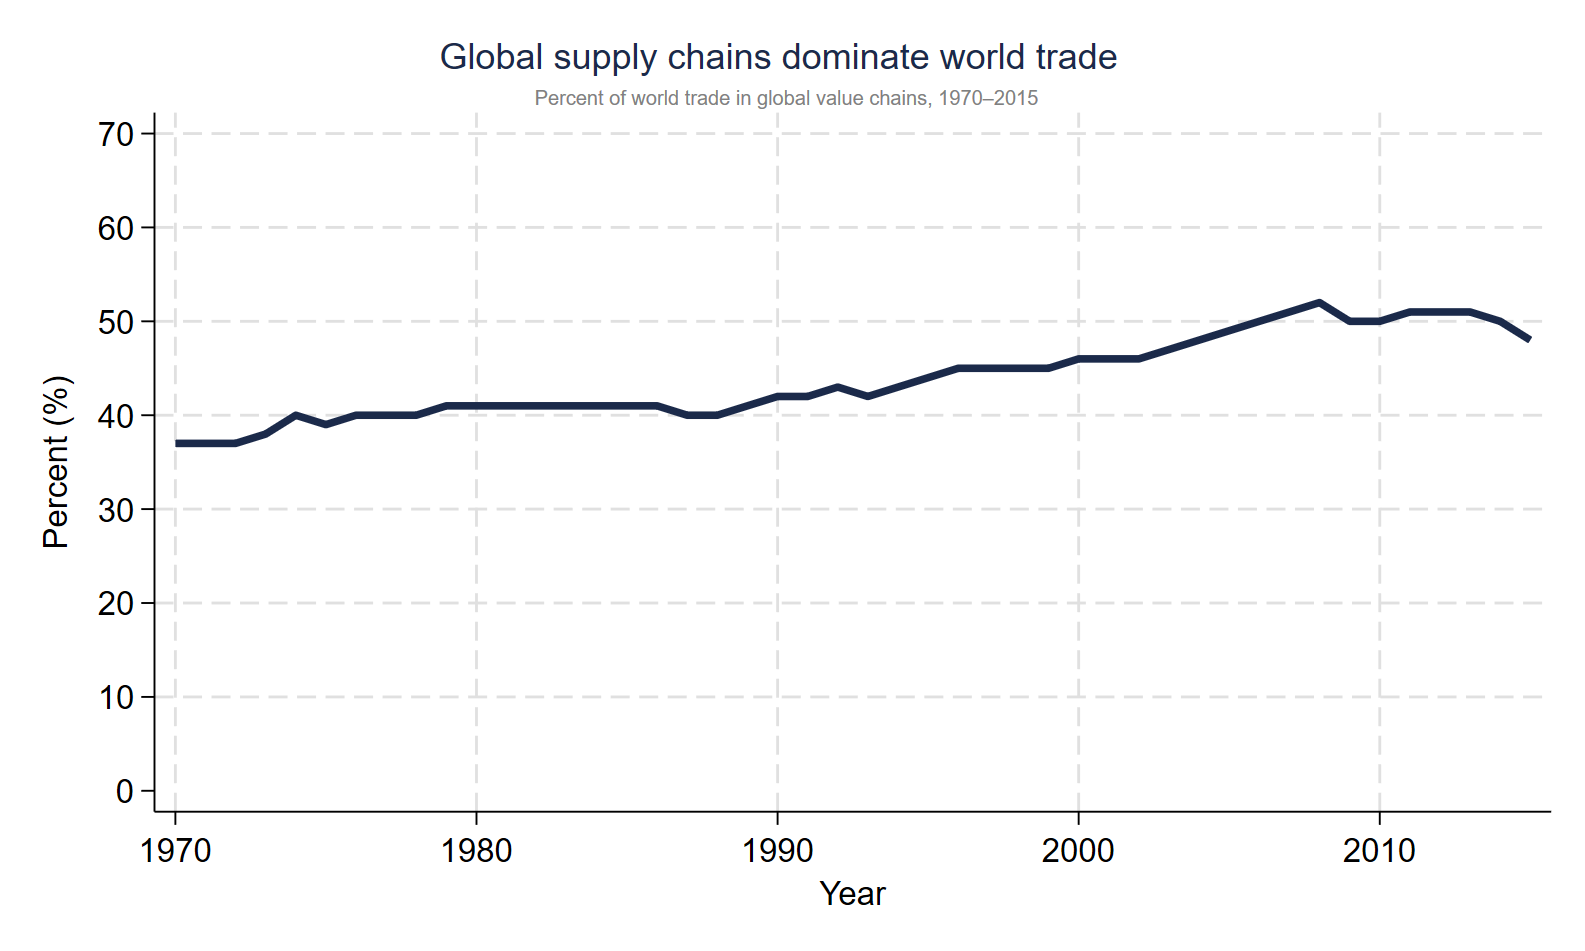
\includegraphics[width=0.98\linewidth, height=0.82\textheight, keepaspectratio]{pic_5.png}
    \end{center}
    \vfill
    {\tiny \color{CustomGray}\textbf{Source:} World Development Indicators (WDI).}
\end{frame}
\begin{frame}
    \vspace{-0.2cm}
    \begin{center}
        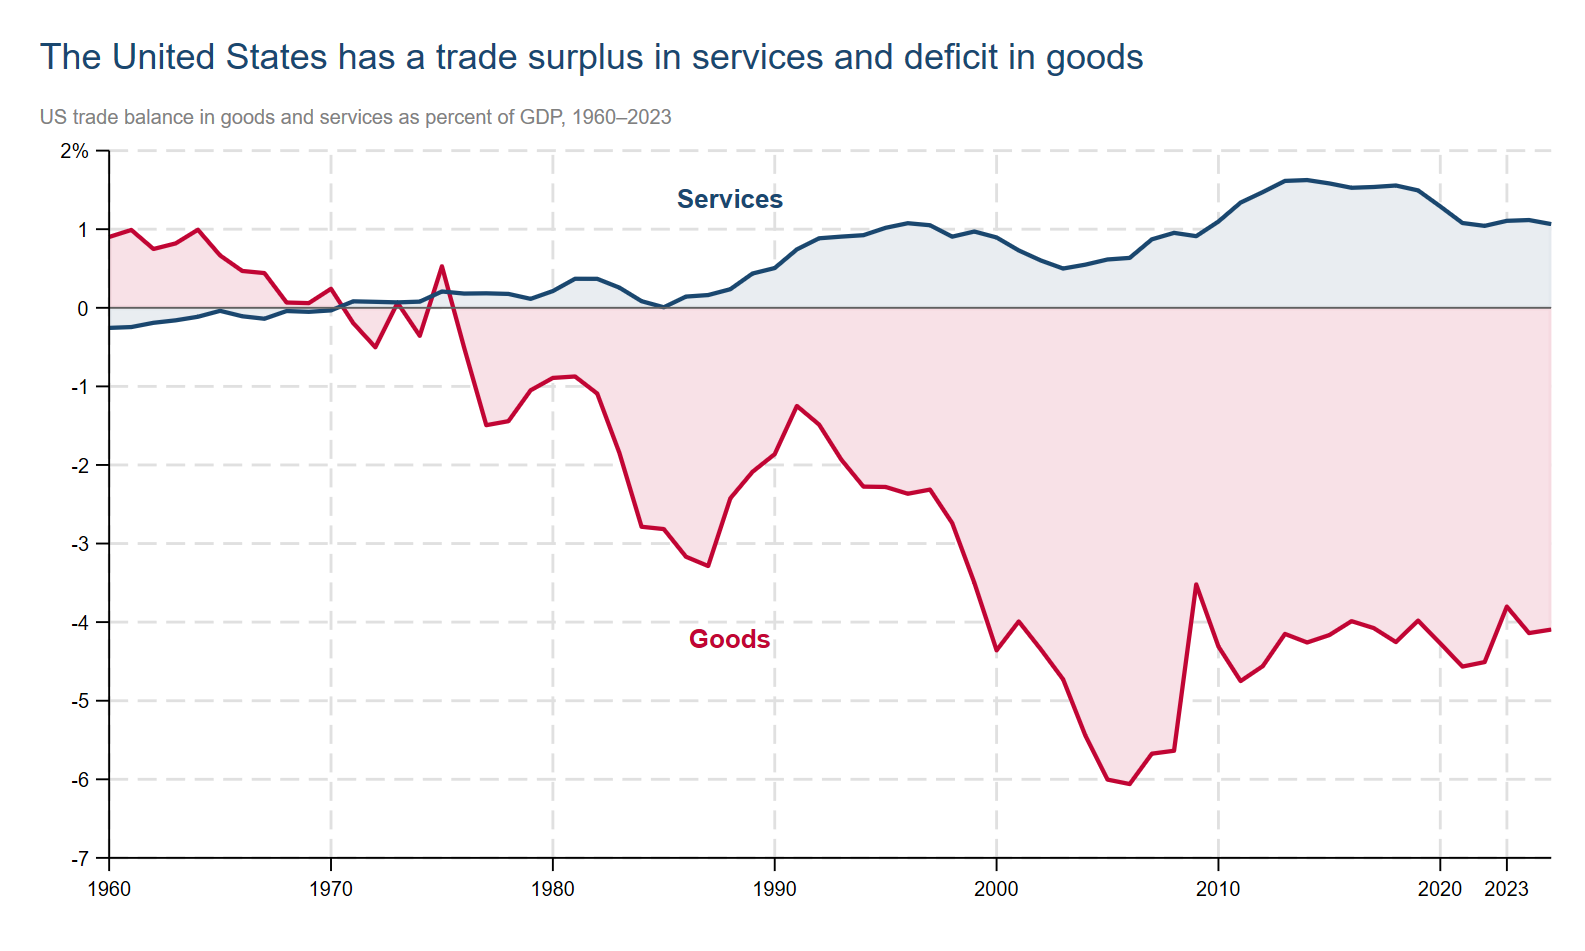
\includegraphics[width=0.98\linewidth, height=0.82\textheight, keepaspectratio]{pic_6.png}
    \end{center}
    \vfill
    {\tiny \color{CustomGray}\textbf{Source:} US Bureau of Economic Analysis.}
\end{frame}
\begin{frame}
    \vspace{-0.2cm}
    \begin{center}
        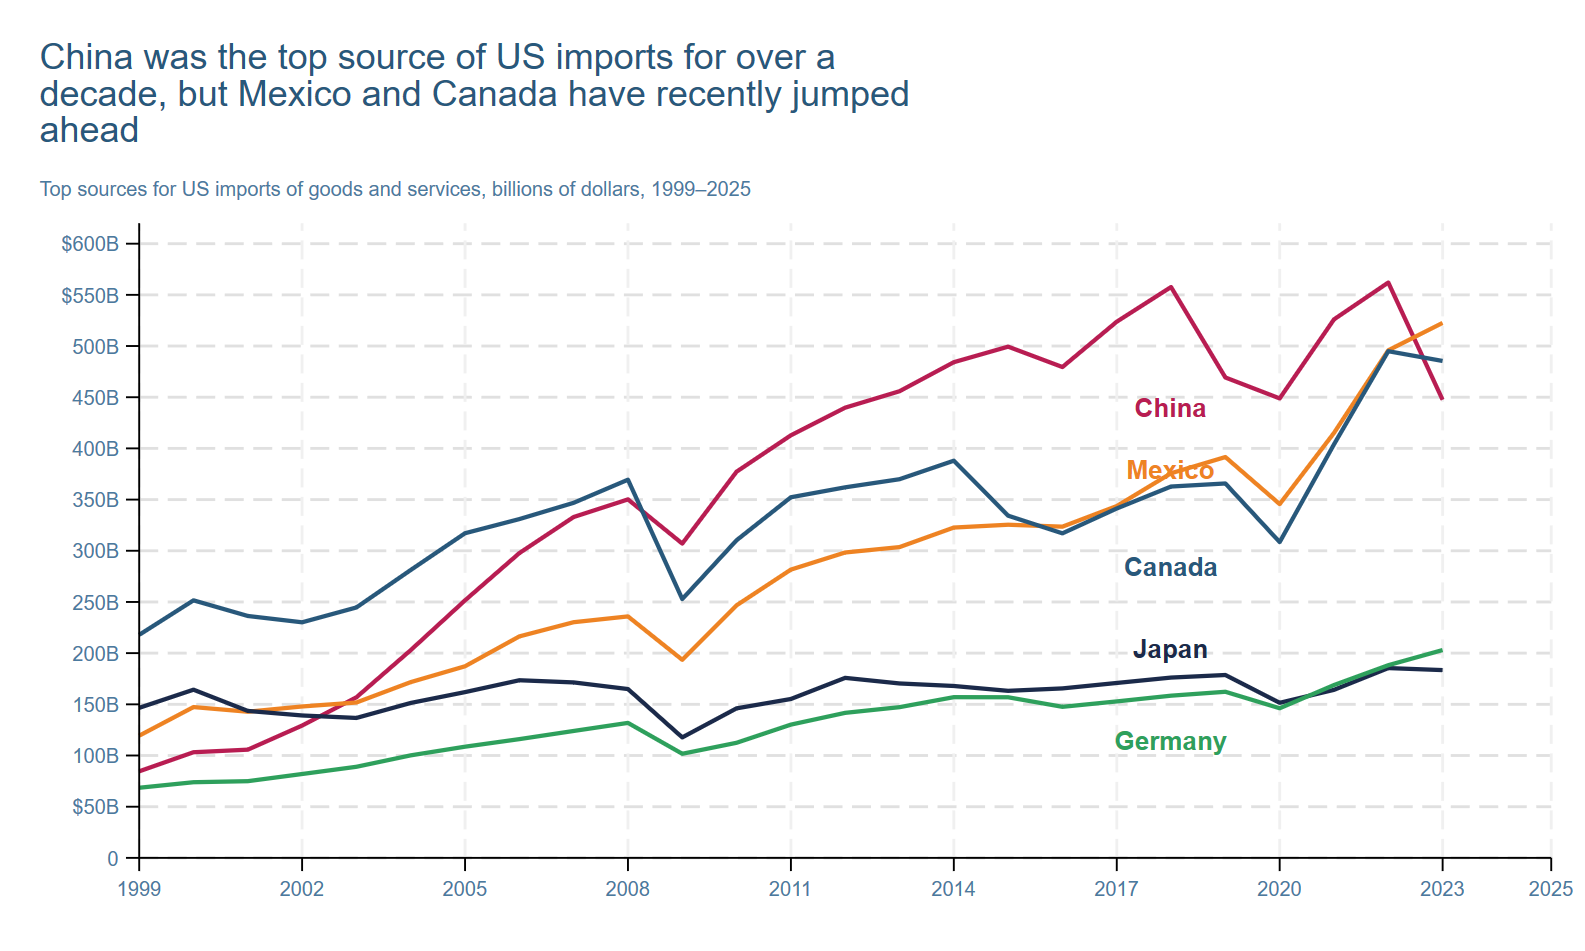
\includegraphics[width=0.98\linewidth, height=0.82\textheight, keepaspectratio]{pic_7.png}
    \end{center}
    \vfill
    {\tiny \color{CustomGray}\textbf{Source:} US Bureau of Economic Analysis.}
\end{frame}
\begin{frame}
    \vspace{-0.2cm}
    \begin{center}
        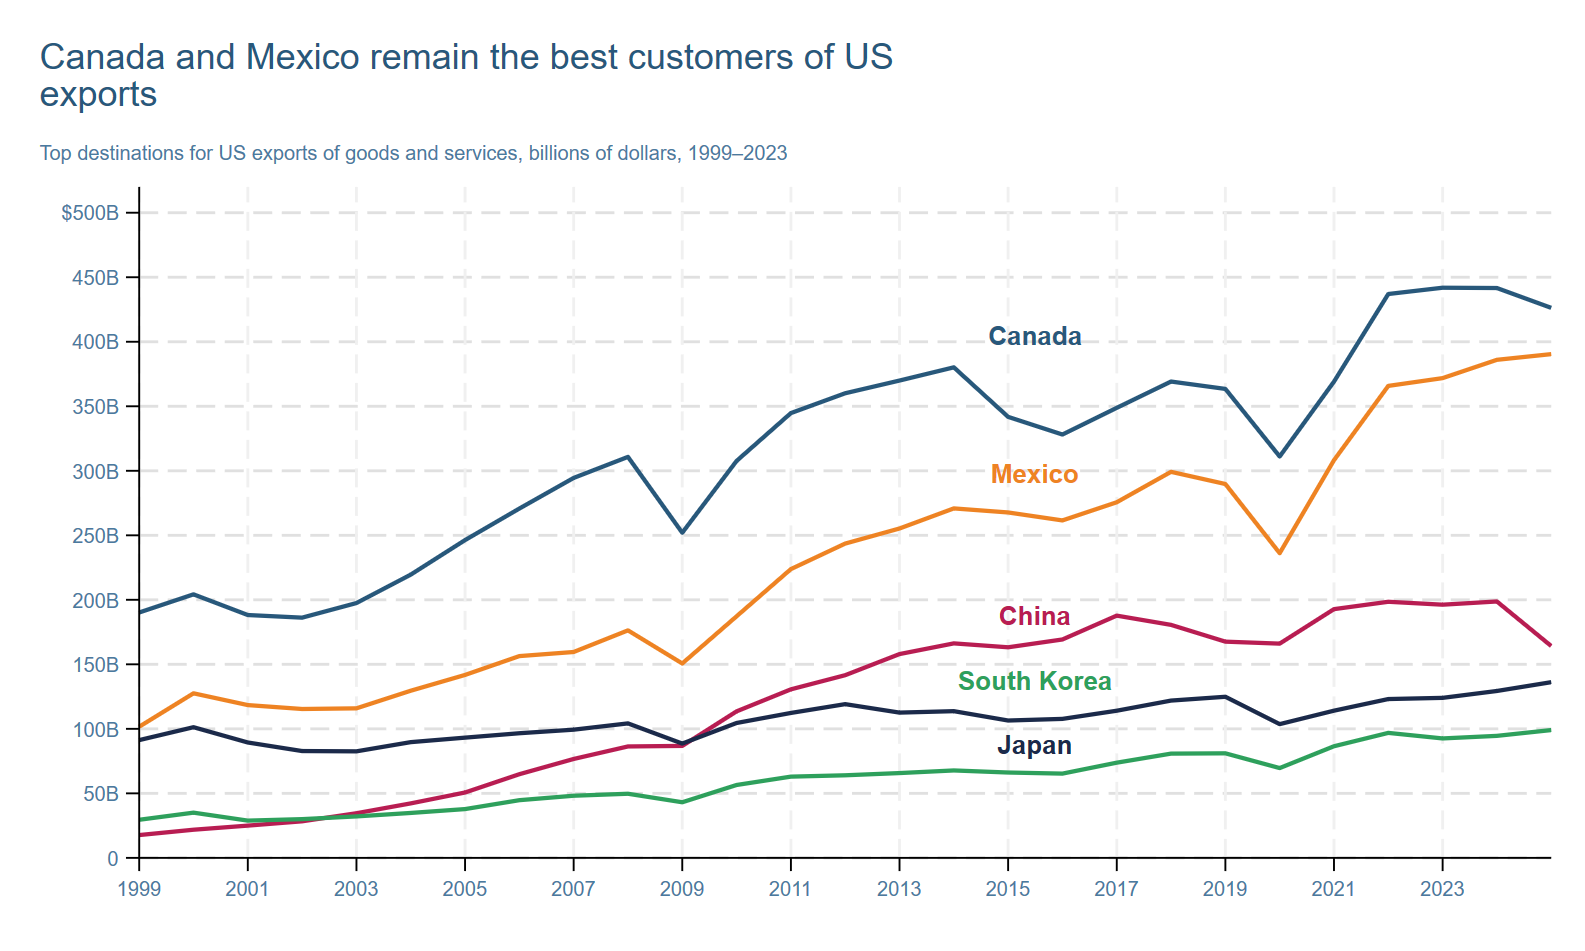
\includegraphics[width=0.98\linewidth, height=0.82\textheight, keepaspectratio]{pic_8.png}
    \end{center}
    \vfill
    {\tiny \color{CustomGray}\textbf{Source:} US Bureau of Economic Analysis.}
\end{frame}
\begin{frame}
    \vspace{-0.2cm}
    \begin{center}
        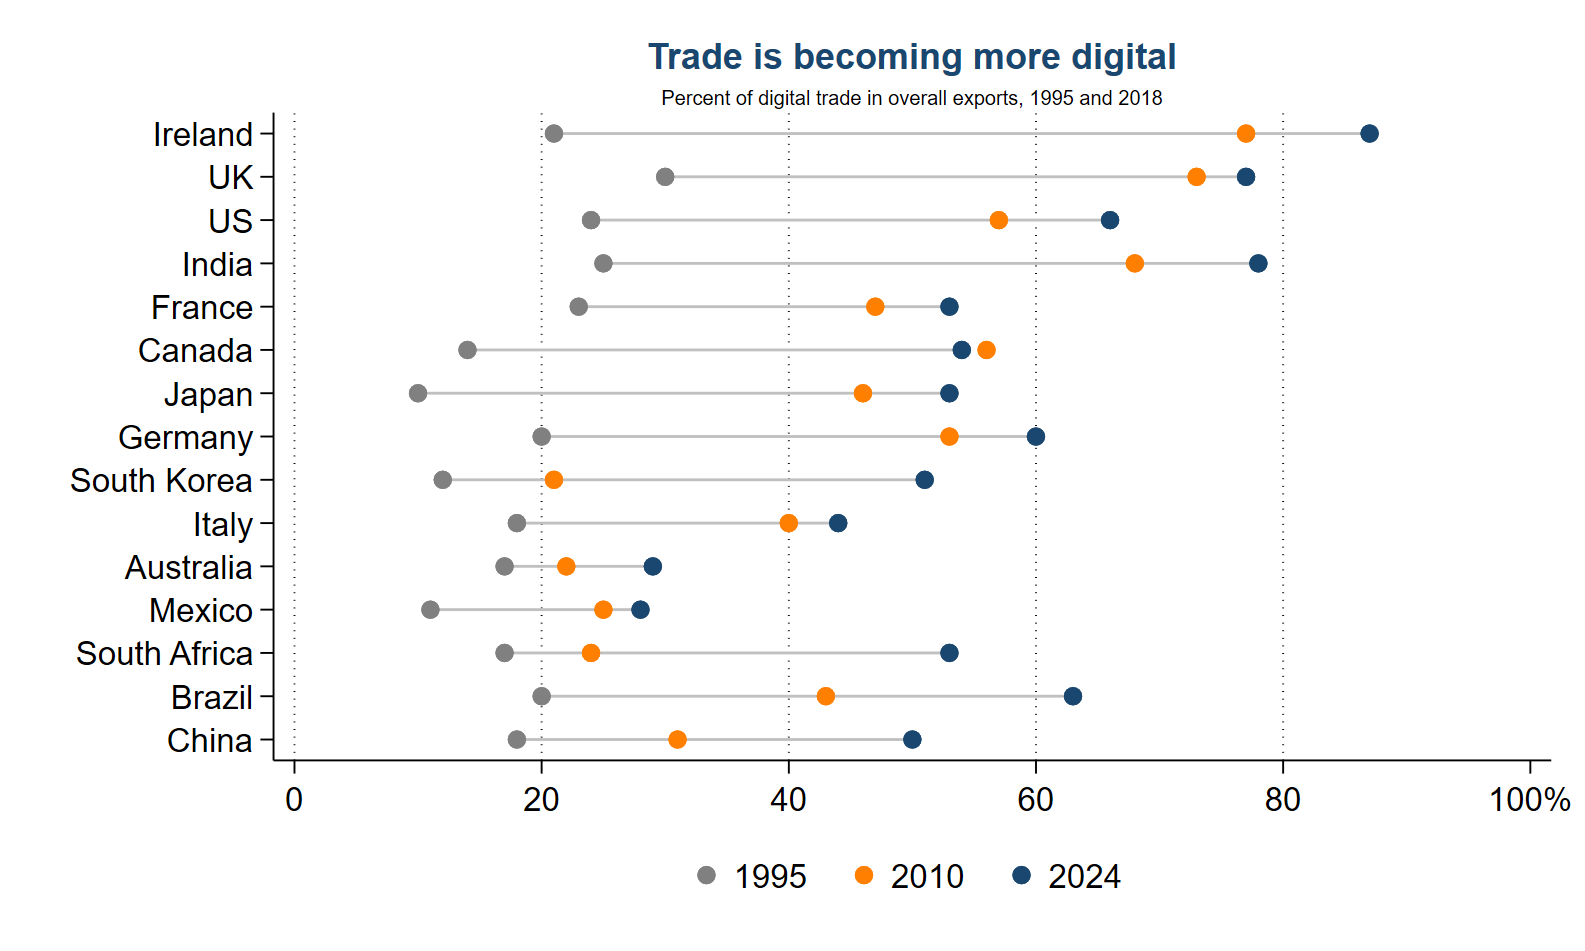
\includegraphics[width=0.98\linewidth, height=0.72\textheight, keepaspectratio]{pic_9.png}
    \end{center}
    \vfill
    {\tiny \color{CustomGray}\textbf{Note:} 1995 Indicators: Digitally deliverable exports as a percentage of total overall trade (Goods + Services). 2010 \& 2024 Indicators: Digitally deliverable services exports as a percentage share of total service exports.\par}
    \vspace{0.05cm}
    {\tiny \color{CustomGray}\textbf{Sources:} 1995 Series: Peterson Institute for International Economics (PIIE) / OECD Trade in Value-Added (TiVA) Database. 2010 \& 2024 Series: UNCTAD-WTO Trade in Services Data Set (Digitally deliverable services: Trade – Annual analytical dataset).}
\end{frame}
\begin{frame}
    \vspace{-0.2cm}
    \begin{center}
        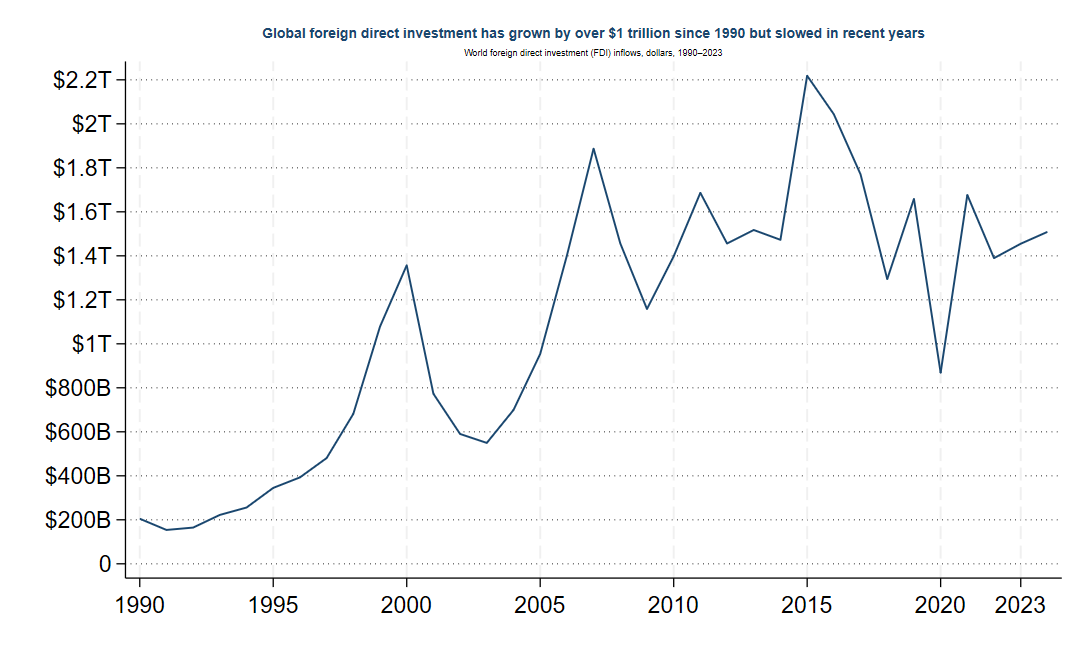
\includegraphics[width=0.98\linewidth, height=0.82\textheight, keepaspectratio]{pic_10.png}
    \end{center}
    \vfill
    {\tiny \color{CustomGray}\textbf{Source:} UNCTADstat Foreign Direct Investment: Inward and outward flows.}
\end{frame}
\begin{frame}
    % Main Heading & Subheading
    {\large \textbf{The United States has been the biggest driver of foreign direct investment for several decades}}\par
    \vspace{0.05cm}
    {\small \color{CustomGray}Top economies for foreign direct investment (FDI), billions of dollars, 1990--2023}\par
    \vspace{0.15cm}
    % Graphs Side by Side
    \begin{columns}[c]
        % Left Column: FDI Inflow
        \begin{column}{0.49\textwidth}
            \centering
            {\small \textbf{FDI Inflow}}\par\vspace{0.08cm}
            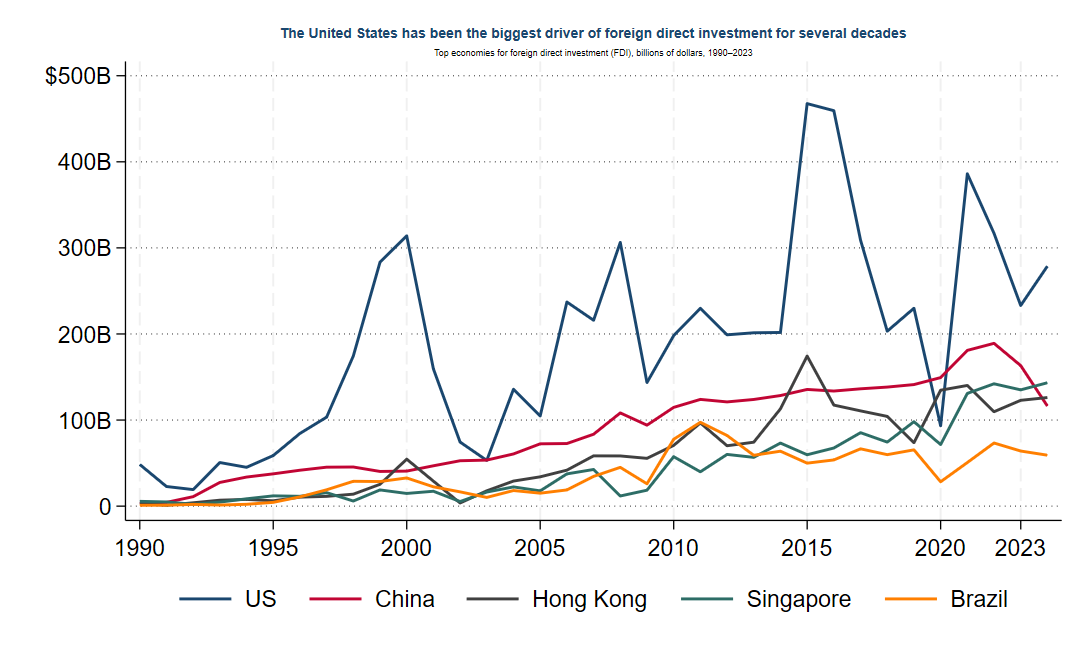
\includegraphics[width=\linewidth, height=0.65\textheight, keepaspectratio]{pic_11.png}
        \end{column}
        % Right Column: FDI Outflow
        \begin{column}{0.49\textwidth}
            \centering
            {\small \textbf{FDI Outflow}}\par\vspace{0.08cm}
            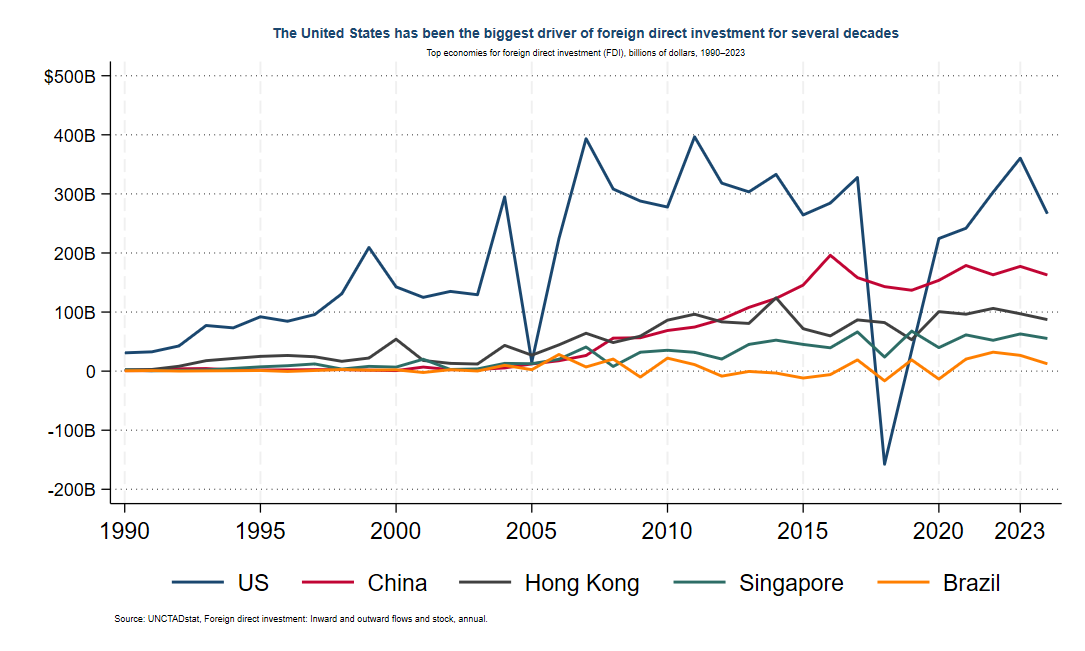
\includegraphics[width=\linewidth, height=0.65\textheight, keepaspectratio]{pic_11b.png}
        \end{column}
    \end{columns}
    % Data Source
    \vfill
    {\tiny \color{CustomGray}\textbf{Source:} UNCTADstat, "Foreign direct investment: Inward and outward flows and stock, annual," UN Trade \& Development Data Hub.}
\end{frame}
\begin{frame}
    \vspace{-0.3cm}
    \begin{center}
        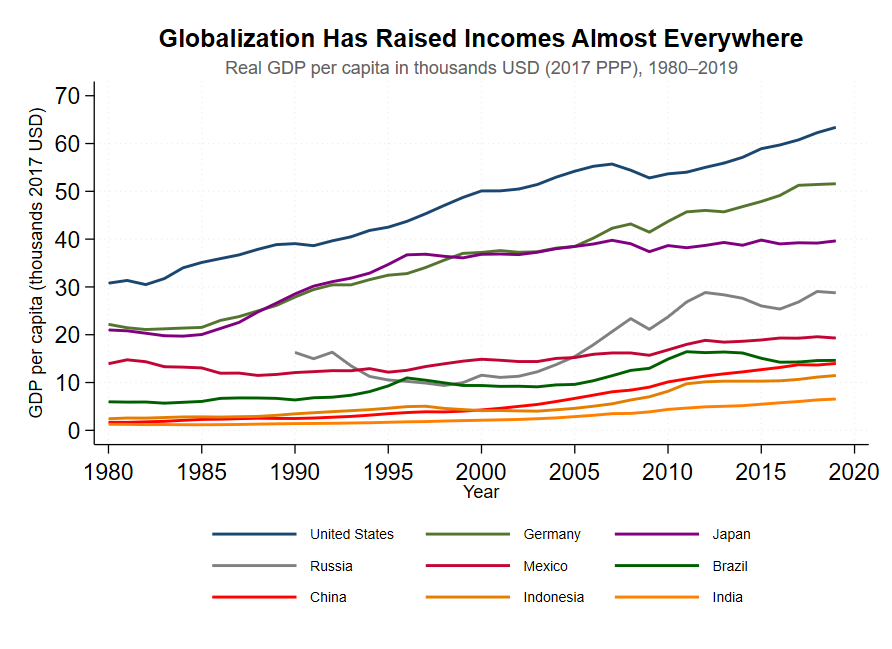
\includegraphics[width=1.0\linewidth, height=0.78\textheight, keepaspectratio]{pic_12.png}
    \end{center}
    \vfill
    {\tiny \color{CustomGray}\textbf{Note:} GDP refers to expenditure-side real GDP at chained purchasing power parity (PPP) rates in 2017 US dollars (rgdpe / pop).\par}
    \vspace{0.05cm}
    {\tiny \color{CustomGray}\textbf{Source:} Penn World Table, version 10.01 (Feenstra, Inklaar, and Timmer, 2015).}
\end{frame}
\begin{frame}
    \vspace{-0.2cm}
    \begin{center}
        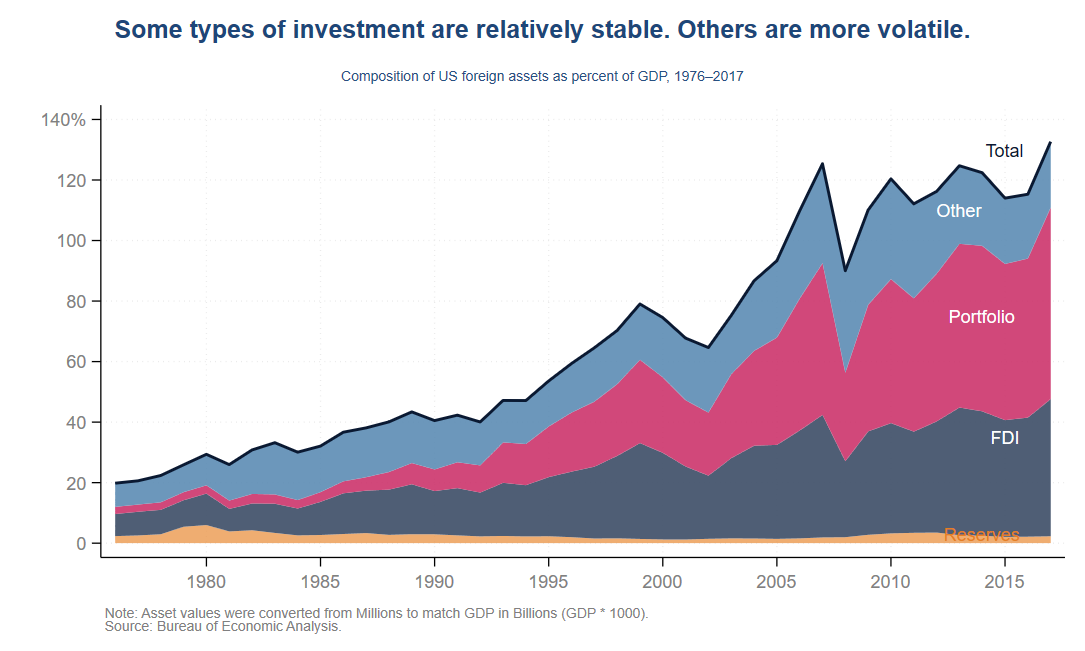
\includegraphics[width=0.98\linewidth, height=0.88\textheight, keepaspectratio]{pic_13.png}
    \end{center}
\end{frame}
\begin{frame}
    \vspace{-0.2cm}
    \begin{center}
        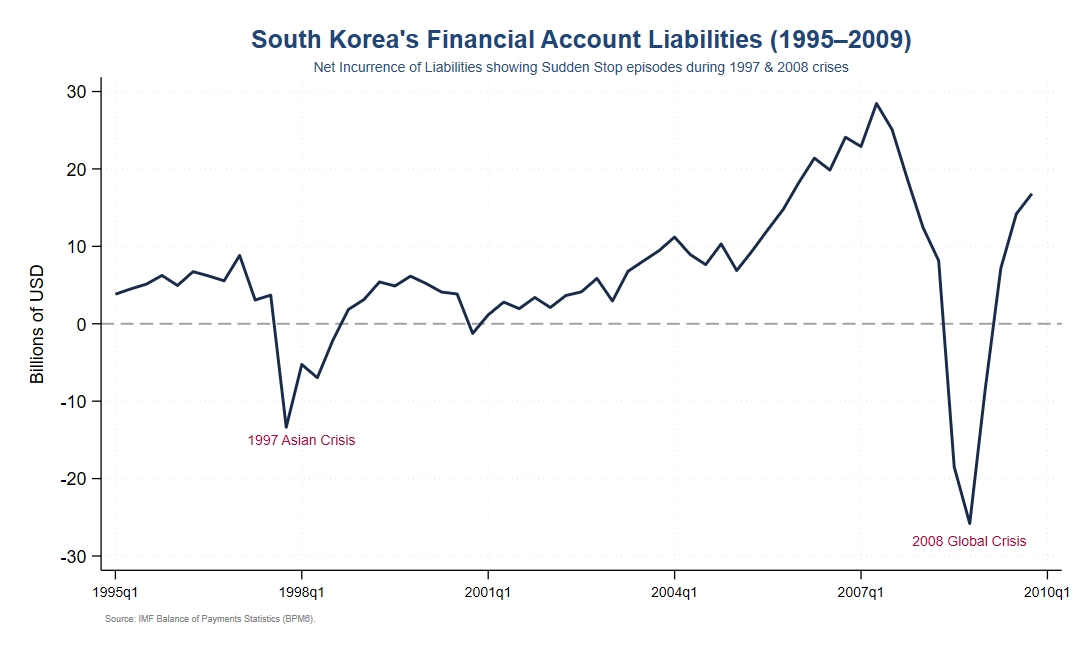
\includegraphics[width=0.98\linewidth, height=0.88\textheight, keepaspectratio]{pic_14.png}
    \end{center}
\end{frame}
\begin{frame}[t]
    \frametitle{GLOBALIZATION AS A TOOL FOR PROSPERITY AND PEACE}
    \vfill
    \begin{itemize}
        \setlength{\itemsep}{0.5cm}
        \item The post-WWII institutional framework - comprising the IMF, World Bank, WTO, UN, and NATO establishes rules-based governance across macroeconomic stability, multilateral trade, development, and security.
        \item This architecture lowers international transaction costs, hedges systemic risks, and stabilises global economic integration to sustain long-run growth and peace.
    \end{itemize}
    \vfill
\end{frame}
\begin{frame}[t]
    \frametitle{EFFECTS OF GLOBALIZATION}
    \vspace{0.2cm}
    \begin{itemize}
        \setlength{\itemsep}{0.25cm}
        {\small
        \item Comparative advantage optimizes resource allocation, lowering marginal production costs and raising real purchasing power.
        \item Broader market access amortizes fixed capital and R\&D expenditures over larger volume, maximizing scale efficiencies.
        \item Foreign competition squeezes domestic markups, incentivizing product innovation and broadening consumer choice.
        \item International trade accelerates cross-border technology spillovers and the adoption of frontier ideas.
        \item Trade induces structural labor reallocation toward high-skill export sectors rather than altering aggregate unemployment, though localized manufacturing displacement occurs.
        \item Globalization compresses cross-country income disparities while marginally widening domestic wage inequality, accounting for 10--20\% of US wage dispersion.
        }
    \end{itemize}
\end{frame}
\begin{frame}[t]
    \frametitle{GLOBALIZATION HAS DISPLACED SOME WORKERS, WHILE SUPPORTING HIGH-SKILL JOBS}
    \vfill
    \begin{itemize}
        \setlength{\itemsep}{0.35cm}
        {\small
        \item Globalization changes the types of jobs available rather than net employment, shifting demand from trade-exposed manufacturing to high-skill services.
        \item Import competition caused severe, long-term wage losses for lower-skilled manufacturing workers while eroding overall labor bargaining leverage.
        \item Workers in high-skill service sectors and foreign-owned companies operating in the US benefited through rapid job growth and significantly higher pay.
        \item Preparing the workforce for expanding sectors like technology, healthcare, and professional services requires targeted job training and higher education.
        }
    \end{itemize}
    \vfill
\end{frame}
\begin{frame}[t]
    \frametitle{WHAT HAS HAPPENED TO AMERICAN MANUFACTURING EMPLOYMENT?}
    \vspace{-0.2cm}
    \begin{columns}[c]
        % Left Column - Figure 1
        \begin{column}{0.49\textwidth}
            \centering
            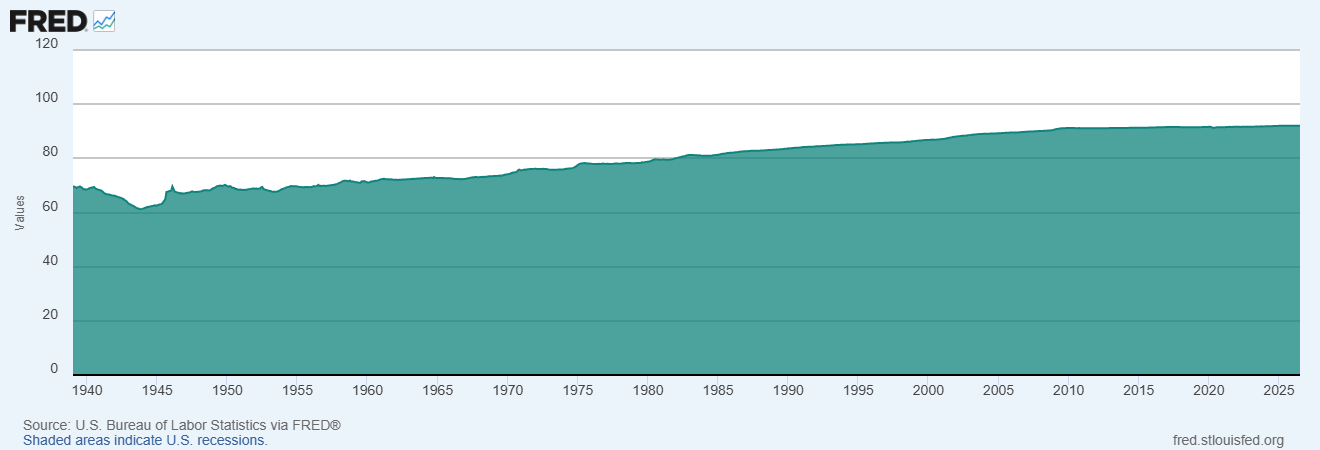
\includegraphics[width=1.0\linewidth, height=0.58\textheight]{pic_15.png}
            \vspace{0.08cm}
            {\tiny
            \textbf{Figure 1: Share of US Employment (Jan 1939--Jul 2022)}\\
            Since World War II, American jobs have increasingly been in service-providing industries instead of manufacturing.\\
            \textit{Notes: Green area represents Nonmanufacturing; white area represents Manufacturing. Nonmanufacturing includes mining, logging, construction, service-providing, and government.}\\
            \textit{Source: FRED, St. Louis Fed.}
            }
        \end{column}
        % Right Column - Figure 2
        \begin{column}{0.49\textwidth}
            \centering
            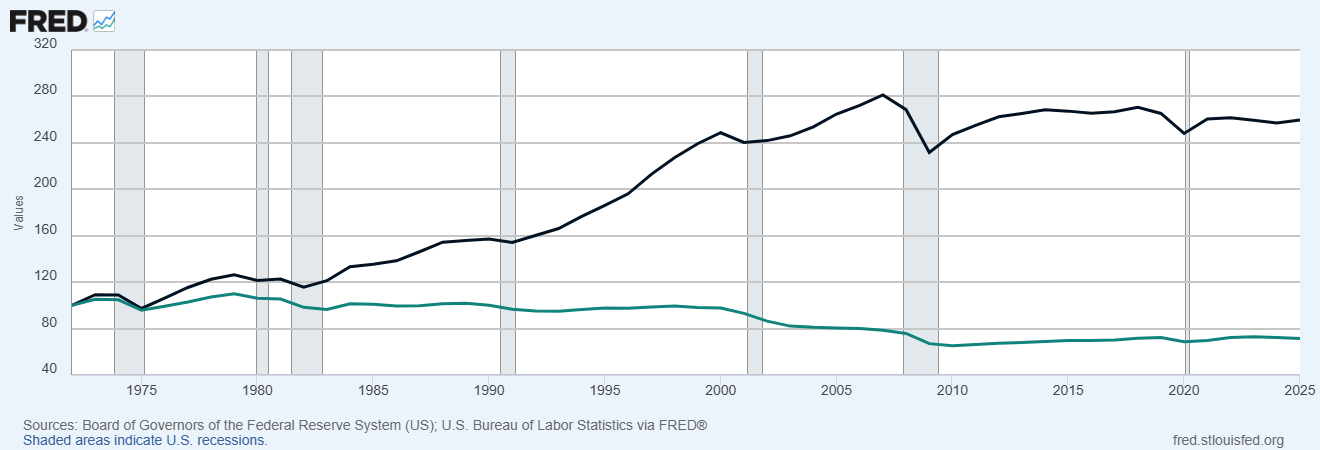
\includegraphics[width=1.0\linewidth, height=0.58\textheight]{pic_16.png}
            \vspace{0.08cm}
            {\tiny
            \textbf{Figure 2: US Production and Employment (1972--2021)}\\
            US manufacturing production needs fewer employees to sustain output than in previous decades (Index, 1972 = 100).\\
            \textit{Notes: Dark blue line represents Production; green line represents Employees. Data are seasonally adjusted. Annual values are averages of monthly data.}\\
            \textit{Source: FRED, St. Louis Fed.}
            }
        \end{column}
    \end{columns}
\end{frame}
\begin{frame}[t]
    \frametitle{WHY SUPPORT GLOBALIZATION IF IT DISPLACES JOBS?}
    \vfill
    \begin{itemize}
        \setlength{\itemsep}{0.35cm}
        {\small
        \item Aggregate economic gains and overall welfare significantly outweigh localized displacement, functioning much like productivity-enhancing technological progress.
        \item Protectionist measures like tariffs protect select industries at a severe cost to consumers, downstream businesses, and retaliatory export sectors.
        \item Staying out of global trade integration isolates domestic firms, lowers real national income, and penalizes competitiveness against foreign supply chains.
        \item Rules-based economic integration strengthens geopolitical alliances and provides institutional frameworks to resolve trade disputes peacefully.
        }
    \end{itemize}
    \vfill
\end{frame}
\begin{frame}[t]
    \frametitle{HOW CAN THE UNITED STATES HELP WORKERS FIND NEW JOBS WITHOUT SACRIFICING TRADE GAINS?}
    \vfill
    \begin{itemize}
        \setlength{\itemsep}{0.35cm}
        {\small
        \item Aggregate national income gains from expanded trade exceed worker adjustment costs by more than tenfold, providing ample resources to compensate displaced workers while preserving trade benefits.
        \item Comprehensive safety net policies—such as wage insurance, expanded tax credits, and subsidized health coverage—can cushion job transitions caused by both trade competition and broader market shifts.
        \item Existing US support through Trade Adjustment Assistance (TAA) remains narrowly targeted and limited, with active labor market spending at just one-fifth the average of other advanced economies.
        \item Strengthening long-term workforce adaptability requires broader investments in education and public healthcare, aligning domestic safety nets with international standards of open-market economies.
        }
    \end{itemize}
    \vfill
\end{frame}
\begin{frame}[t]
    \frametitle{CHINA'S RISE IN THE GLOBAL ECONOMY CREATES COMPLICATED PROBLEMS}
    \vfill
    \begin{itemize}
        \setlength{\itemsep}{0.35cm}
        {\small
        \item China's post-WTO integration created systemic trade frictions through state subsidies, forced technology transfers, and non-market policies that disadvantage foreign competitors.
        \item Multilateral strategies aimed at reforming Chinese practices—such as the original TPP framework and joint EU-US-Japan WTO initiatives—were disrupted by US strategic pivots toward unilateral protectionism.
        \item The bilateral trade war escalated average tariffs to ~20\%, shifting costs directly onto importing firms and consumers without resolving structural issues or eliminating the overall US trade deficit.
        \item Unilateral protectionist measures—including tit-for-tat tariffs, TPP withdrawal, and 'Buy America' mandates—fragment global supply chains, erode rules-based WTO governance, and risk severe economic retaliation.
        }
    \end{itemize}
    \vfill
\end{frame}
\begin{frame}[t]
    \frametitle{THE PUBLIC HAS MIXED VIEWS ON GLOBALIZATION}
    \vfill
    \begin{itemize}
        \setlength{\itemsep}{0.35cm}
        {\small
        \item Public perception of globalization is split because diffuse consumer benefits are less visible than concentrated, localized job losses among specific communities.
        \item Political friction is amplified by inadequate domestic adjustment policies and growing income inequality during periods of rapid global integration.
        \item Demographic trends show stronger support for free trade among younger generations who came of age within an integrated global economy.
        \item Traditional political alignment shifted after 2016 as executive trade policy pivoted toward protectionism, renegotiating key agreements like NAFTA into the USMCA.
        }
    \end{itemize}
    \vfill
\end{frame}
\begin{frame}[t]
    \frametitle{SUSTAINING GLOBALIZATION THROUGH POLICY ACTION}
    \vfill
    \begin{itemize}
        \setlength{\itemsep}{0.35cm}
        {\small
        \item Updating multilateral frameworks through rules-based negotiations is necessary to address digital commerce, unfair subsidies, and sectoral trade disputes without escalating into destructive trade wars.
        \item Comprehensive domestic policies targeting job training, healthcare affordability, and wage growth are essential to mitigate displacement caused by both trade integration and rapid technological automation.
        \item Ensuring inclusive economic growth and robust social safety nets protects broad national well-being while preventing the erosion of rules-based international institutions.
        \item Accessing the 95\% of global consumers outside the US requires maintaining reciprocal open market access to preserve international competitiveness and capture substantial real income gains.
        }
    \end{itemize}
    \vfill
\end{frame}
\begin{frame}[t]
    \frametitle{POLICY RECOMMENDATIONS}
    \vfill
    \begin{itemize}
        \setlength{\itemsep}{0.35cm}
        {\small
        \item Invest in inclusive education, active job retraining, wage insurance, and portable healthcare benefits to enhance workforce adaptability and cushion transition costs for displaced workers.
        \item Mitigate widening income inequality and support vulnerable households through progressive tax reforms, targeted transfer programs, and expanded social safety nets.
        \item Leverage high-standard free trade agreements to enhance domestic business competitiveness, expand market access, and drive long-term macroeconomic growth.
        \item Reform and strengthen rules-based institutions like the WTO alongside international allies to settle disputes, enforce intellectual property rights, and counter unfair trade practices.
        }
    \end{itemize}
    \vfill
\end{frame}
\begin{frame}[t]
    \frametitle{REFERENCES}
    \vfill
    \begin{itemize}
        \setlength{\itemsep}{0.35cm}
        {\small
        \item Peterson Institute for International Economics. (2024, August 16). \textit{What is globalization?} https://www.piie.com/microsites/globalization/what-is-globalization.
        }
    \end{itemize}
    \vfill
\end{frame}
	
\end{document}
